\chapter{What is Context?}

This chapter describes what we mean by `Context' and `Context-Awareness'. We look at the previous definitions and usages of these terms, and propose why these are lacking for the purposes of this dissertation. As we go through each definition, we will pick out the most relevant parts to form the ground for the context framework introduced in this and developed in later chapters.

\section{Previous Definitons}

The earliest study on context was done by Bill Schilit in 1994, and reported in their paper [CITE]. The focus in this study was how to build software in dynamic environments. The dynamics of the environments were largely due to people requiring computational services, the modality of request (through a mobile device or through a workstation), and the environment of the device (are there cameras and projectors nearby if the task requires video conferencing?). This software-centric view of context highlights the importance of two things. One, context is always described with respect to an object. In this case it is the software which runs on processors distributed in a real world environment. Second, context is used to determine how this object interacts with events and entities near it? For example, Schilit uses the example that a workstation should automatically load his favorite text editor when he approaches it; and an rooster music sample must be played whenever fresh coffee is prepared. Both very different and precise interactions even though they might share common background (environment or participating entities). We would not expect a text editor to be shown when coffee is prepared, and the rooster music to be played when an employee walks to a workstation.

In his seminal paper, Anind Dey [CITE] describes context \textit{as any information that can be used to characterize the situation of an entity. An entity is a person, place or object that is considered relevant to the interaction between a user and an application, including the user and applications themselves.} He proceeds to explain this definition with the example of an ``indoor mobile tour", arguing that there are there are two additional pieces of information which can be used: \textit{weather} and \textit{presence of other people}. if the user is present with his friends, they might visist sites that are of interest to everybody. There the presence of other people is important context. Because the tour is indoor, weather does not affect the application. It is true that the weather has no direct affect on the application but what about the following scenarios:

\begin{itemize}
\item Could we use the weather information to serve different drinks in the cafeteria? On a cold day, placing the hot chocolate kiosk next to the entrance and the ice cream kiosk closer on a warmer day might boost some sales? And add to the overall experience of the tourists?
\item If the tour is similar to Alcatraz, where a ferry ride takes people to the island, and back from it, a storm brewing in the ocean could lead to disrputed ferry services. Should the application warn its users who are liesurely touring at this time? Or should they continue the tour at the same pace, miss the last ferry and spend the night at Alcatraz? After all, accommodation is not a problem.
\end{itemize}

They then proceed to define Context-Aware computing as follows: \textit{A system is context-aware if it uses context to provide relevant information and/or services to the user, where relevancy depends on the user's tasks}. But, we need to ask ourselves why a system which uses this ``additional information" should be considered a context-aware system. There are numerous system which simply would consider these ``additional information" as regular inputs. What is the different between a system which takes in these inputs as processes them as regular data, and one which processes them as context?

Karen Henricksen [CITE] makes the following interesting observation about context: Context information exhibits a range of temporal characteristics. Some context information can be static, for example the attributes of people using a system (for example, the sex of a person). But a large amount of information is dynamic. For example, relations change between people, location and events progress between moments. There is no straightforward way to obtain this dynamic information other than through sensors. But, such a approach tightly couples the application logic to the types of sensors used, and requires the system to convert the input data to usable representations. For example, the application might explicit modules to convert GPS coordinates to readable addresses. The problem with such an approach is that there are many ad-hoc modules built to tackle the sensors, and therefore causing the context-awareness to be tied to a specific application.

More recently, Vaninha Vieira [CITE] uses a knowledge centric view of context to design their context sensitive system, Cemantika. Vaninha defines a contextual element as any piece of data or information which can be used to characterize an entity in an application domain, whereas the context of an interaction between an agent and an application is the set of instantiated contextual elements that are necessary to support the task at hand. Context awareness, for them, is to explicitly change the task which the system is carrying out. For this they explictly model the \textit{context sources} which includes heterogenous and  external sources like sensors, user dialog interfaces and databases. This allows the various processes to operate independently of the type of sources. It should be noted that the use of ontologies is describing knowledge and context sources is becoming increasingly popular. A more listing of relevant work is provided in chapter 3. \textbf{This paves the way for us to bring in the notion of types of information}.

Let us extend the tour guide example to demonstrate the different properties of context. In this extension, we assume that this is the tour guide software to manage a visitor's experience at the Alcatraz Island, San Francisco. The visitor is allowed to walk through the exhibits as s/he pleases, with the tour guide headset providing explanations on the current exhibit, by sensing the current location. The explanations provided are such that they take into consideration what the visitor has already seen at the prison. For example, if the current location requires knowledge of an event which happened at a different section of the prison, then it must not be told. The application must also ensure that all visitors make it to a ferry ride before the last one departs for the day. If there is any problem in that respect, it must present the appropriate data which informs the visitor on the reason for the problem. Since this application knows where every visitor is at a given time, it must ensure that some sections of the Island do not get more crowded that the others. It should either slow down or move the visitors faster if the number of people in a section are increased beyond a particular threshold.

\begin{figure}[t]
\centering
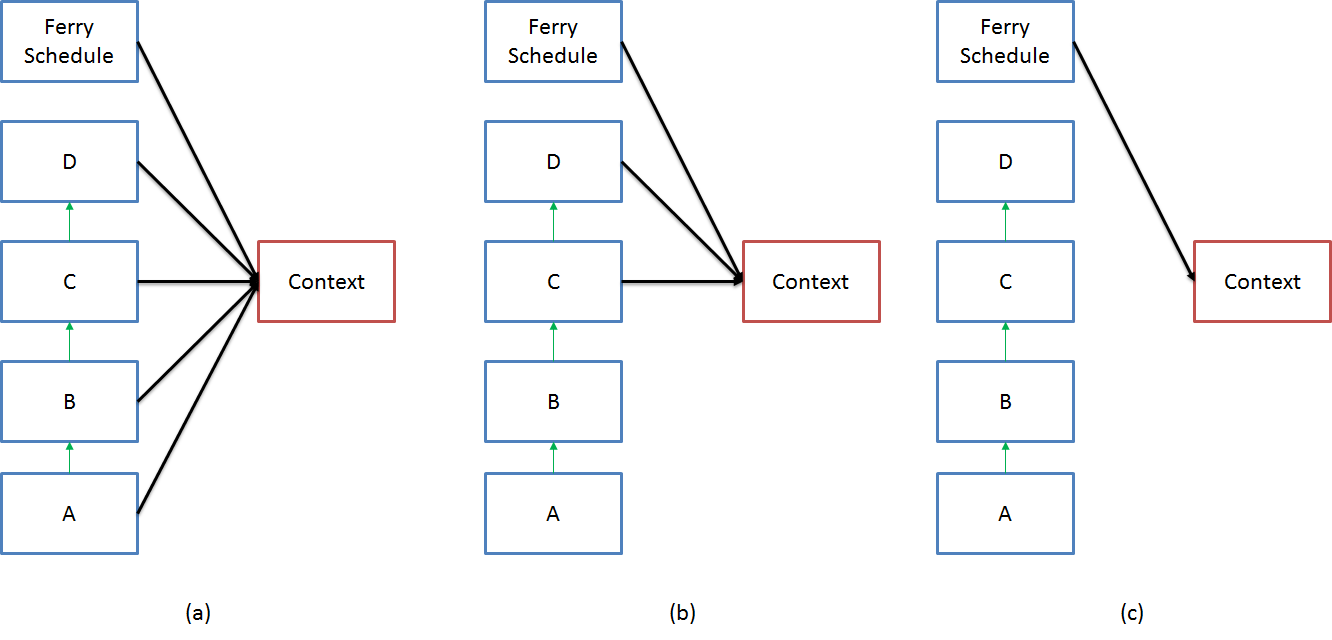
\includegraphics[width=\textwidth]{media/chapter2/changes.png}
\caption{The set of items which contributes relevant context changes as the relations of the primary object with them change.}
\label{fig:turkey}
\end{figure}

Let's assume that the Island is divided into sections, each of which contains a person counter sensor. The counter sensor can be queried to determine how many people are present in the section. Each visitor carries a handheld device which is capable of sensing its location, and proximity to an exhibit. The ferry maintains a schedule, which is read by the system to make decisions. If there is a problem with the ferry, a maintenance schedule which can be queried to check for any damages to the ferry. We also assume we have access to a local weather channel to check for sudden changes in the weather which might affect the ferry.

When a visitors enters the museum, all sensors are contributing towards the context of the visitor. The person counters are being queried to decide which section the user should move to next, the previous locations are used to form coherent explanations at each new stop. The ferry schedule is checked to make sure there are no disruptions along the way. But what happens when the visitor has finished seeing all the exhibits? We can now ignore all the previous locations, and traffic situation at the different sections. Even though these sensors are in the proximity of the visitor, they are no longer needed. And therefore, contribute no useful context. We can also say \textbf{that the relationships between the visitor, and his environment has changed through time}. Thus, it holds to say that the exact configuration of relationships, at that instant of time, is pivotal in deciding what real world information contributes to context, and what is unecessary.

Relationships can be of different types. They can be simple labels like \texttt{friend-of} signifying a social relationship. Or they can more actionable like \texttt{located-at}, which relates a person to a particular location, and therefore causes a particular audio stream to play through the handheld device. This relation is not just a label, it imposes constraints on the properties of objects which it relates. Here, the spatial attributes of the the person and the exhibit must match if they are being related through a \texttt{located-at} attribute. In this dissertation, we will see that such relations, which impose such property constraints are critical in algorithmically determining which information is relevant context.

We define context of a given object at a particular time as \textbf{``the real world information which can be related to the object directly or indirectly through a known set of relationships''}. Context-awareness of a system is its \textbf{``ability to explore different types of information to identify context relevant to the objects in its ecosystem, and using this additional knowledge to reduce the complexity of a given task''}.

\section{Properties of Context}

\subsection{Object Specificity}
Context is always specified with respect to a real world object. This object must be uniquely identifiable in the computational system, and must be an instance of one of the known classes. This object must have some real world attributes. For example, if the object is an event, then the interval during which it occurs, and location of occurence are two real world attributes.

\subsection{Relation Centric View}
We believe that any context is any event or entity which can be \textit{related} to the variables in a problem. It must be noted that focus has now shifted from finding objects which are of a specific type, and that to objects (of any type), but related to the problem variables through specific relationship types.

\subsection{Temporal Relevance}
The relations between problem variables and the context objects must be temporal in nature. There are two advantages to this. First, this allows us to associate different context objects (possibly of different types) to different instances of the problem. Second, real world relations are always temporal in nature. By explicitly modeling time in our definition of context, we are able to incorporate a majority of real world relations, which are very crucial in real world applications.

\subsection{Dynamic Linking}
When a problem uses a fixed set of context objects for all instances, we refer to it as static linking. But here argument would be -- why call it context? and not just a problem which uses an additional set of variables. In this dissertation, we believe that context must be \textbf{dynamically linked} to the problem variables. This follows from the above two points. For example, tagging faces in photos cannot restrict the search space to be just friends of the user on Facebook. 

In summary, we can say that context is any information which can be dynamically related to information present in the given problem, under the accepted spatio-temporal constraints.

\subsection{Context-Awareness}
A context-aware system is one which is able to dynamically link to those sources of information which provide it most relevant context. In the example of the tour guide system, the sensory out of the sensors were gradually ignored, and at the end, only the ferry schedule was considered relevant. In this dissertation, we will see one such way of selecting such information for a specific face tagging application. 

Also, context has been used in many non-real world problems. For instance, in natural language processing [CITE], ranking pages of the web [CITE-pagerank], entity resolution [CITE], face clustering [CITE] and therefore it must not mean that contextual techniques must apply only to real world problems. For the purposes of this dissertation, we ignore the application of context in such problems.

\section{Parallels}
The real world is very big. Modeling it can be a very hard task. Do we really need such large and elaborate models if we are to call our application ``context-aware"? In this section, we look at how \textit{contextual thinking} has helped understand, and in some cases solve, many of the long standing problems in different disciplines. We will start with an anecdotal example, and move to more elaborate examples which demonstrate how to reason in real world problems. The reason for this section is to justify the need for modeling many different types of real world information, which is a pre-requisite for employing context in the way it is justified above. 

\subsection{Black Swans}
In his widely acclaimed book, The Black Swan, Nassim Nicholas Taleb presents many arguments against solely relying on prediction based techniques. Citing examples from stock markets to clinical psychology trials he presents the case that historical evidence is insufficient to position oneself in the future. 

His example of a turkey brings to light an interesting point ``Consider a turkey that is fed every day. Every single feeding will firm up the bird's belief that it is the general rule of life to be fed every day by friendly members of the human race ``looking out for its best interest''. On the afternoon of the Wednesday before Thanksgiving, something unexpected will happen to the turkey. It will incur a revision of belief.''

Any amount of prediction is futile in this case. Taleb plots the graph \ref{fig:turkey} showing the belief of the turkey in mankind. How could the turkey protect itself, yet reaping the benefits of the food given to it? 

From the standpoint of the turkey, the Wednesday event is a Black Swan event. But from the standpoint of the butcher, it is not, since its occurrence is not unexpected.

The simple example shows how new objects bring with them different semantics. And highlights that object relations can be disrupted heavily with even the slight change in relations. The second thing it shows is the need for awareness in the turkey to ``look-out'' for potential causes of harm. This action of being context-awareness is criticial in any real world systems.

Figure shows how the turkey can navigate to various sources to learn how human beings behave. humans ..to.. festivals ..to.. thanksgiving ..to.. role of turkey in thanksgiving ..to.. butcher's profession.

\begin{figure}[t]
\centering
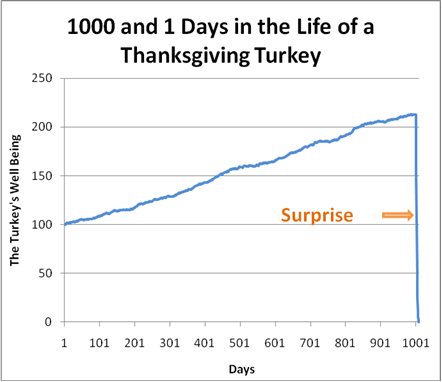
\includegraphics[width=0.75\textwidth]{media/chapter2/turkey.png}
\caption{Expectations of a Turkey as Thanksgiving approaches.}
\label{fig:turkey}
\end{figure}

\subsection{Context in History}
Historians love context. Almost all their works heavily rely on finding interesting events in a particular timeframe which can explain the reasons. In his book, Guns, Germs and Steel, Jared Diamond argues the need to understand specific environmental diversities, and use them to reason why history happened the way it did. We are familiar with the conquest story of the Inca emperor Atahuallpa by the Spanish conquistador Francisco Pizzaro at Cajamarca, Peru in 1532. Historians attribute the success of Pizzaro to better Spanish ammunition and warfare techniques. But the more interesting question is \textit{Why was Pizzaro at Cajamarca conquering the Incas, and not Atahuallpa crossing the Atlantic conquering Spain?}. How did South Americans evolve so different from Europeans? The answer, it turns out, lies in the environment.

Diamond shows the various steps in a flowchart similar to \ref{fig:axis-flowchart}. Lets see how he arrived at this. For a conquest of the Americans, the Europeans needed strong political and economic and  structure, which means separate organizations devoted to monitoring these. The South Americans lacked a political structure. The society consisted of the high ranking chiefs who were treated as Gods, and were the only people permitted to read and write. Everyone else was engaged in food production. In a war, the ability of the Europeans to communicate precise information through the written word was a crucial advantage.

\begin{figure}[t]
\centering
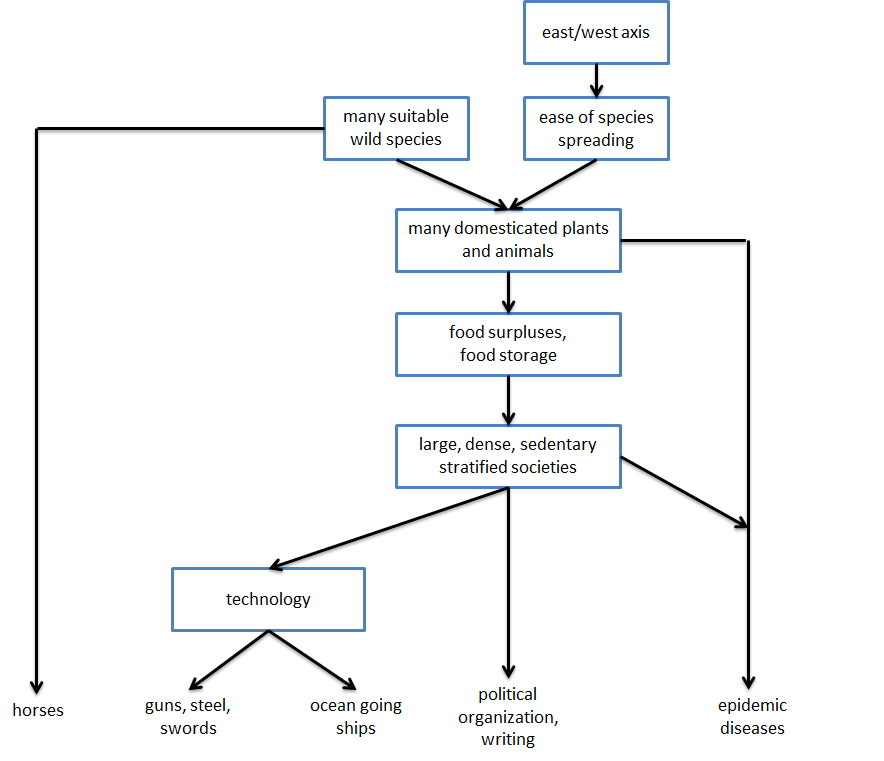
\includegraphics[width=\textwidth]{media/chapter2/axis.png}
\caption{Reasons for diversity among cultures.}
\label{fig:axis-flowchart}
\end{figure}

\textbf{Why did the Europeans form such a stratified society, and not the South Americans?} The majority of the south americans were concerned about procuring food for the next day. Food production systems in Europe reached a critical peak, because of which they developed technology for storing food. Because day-to-day food was no longer a concern, a significant section of the population now was ``free'' to indulge in other activities. This led to development of art, policital, military units, economic systems, which in turn evolved each.

\textbf{Why did food production reach an all time high in Europe and not in South America?} The reason lies in three environmental factors: the soil, flora and fauna of the area and over a larger time span. Europe and Asia has been home to a more diverse set of animals and plans. Since 6000B.C., farmers and animals of the area were able to choose from this bigger variety of plants, and evolve them over thousands of years to form better crops. Big mammals like Cows, Bulls were found in plenty in Europe and Asia. This led to much higher yields than tilling the soil by hand or manually. The role of a larger set of animals in the area is interesting too. Over the years, Europeans have domesticated most of the animals than people from any part of the world (owing to the diversity, animal behavior and the abilities of the animal). For example, there is no point in domesticating an elephant, as it takes 14-15 years to reach adulthood and be of use. Animals like Rhinos can be excellent farm animals owing to their strengths, but are very hard to tame. Areas like Africa were rich in elephants and rhinos but America lacked those too, and both these continents lacked important livestock like cows, bulls and sheep.

\textbf{Finally, why did biodiversity emerge in Europe/Asia, and not in the Americas or Africa?} Thousands of years ago, the biggest deterrent in sustaining life was the climate. People lived nomadic lifestyles which came in contact with different weather, and acclimatizing to it required almost a reboot of their knowledge, environmental know-how and customs. Now, lets take a look at the map of the world, shown in \ref{fig:continental-axis} -- what do we see? Europe and Asia span longitudinally, whereas Americas and Africa extend along Earth's latitude. What is the biggest advantage this offers Eurasians? When they moved from place to place, the structure of their continent allowed them to move to places with \textbf{similar weather}. This allowed them to move to different regions and enjoy the same weather, grow similar crops and domesticate the same animals. But people in Africa or America had to move out of their comfort zone, and move to area containing different weather and biodiversity, and had to redo everything from scratch.

\begin{figure}[t]
\centering
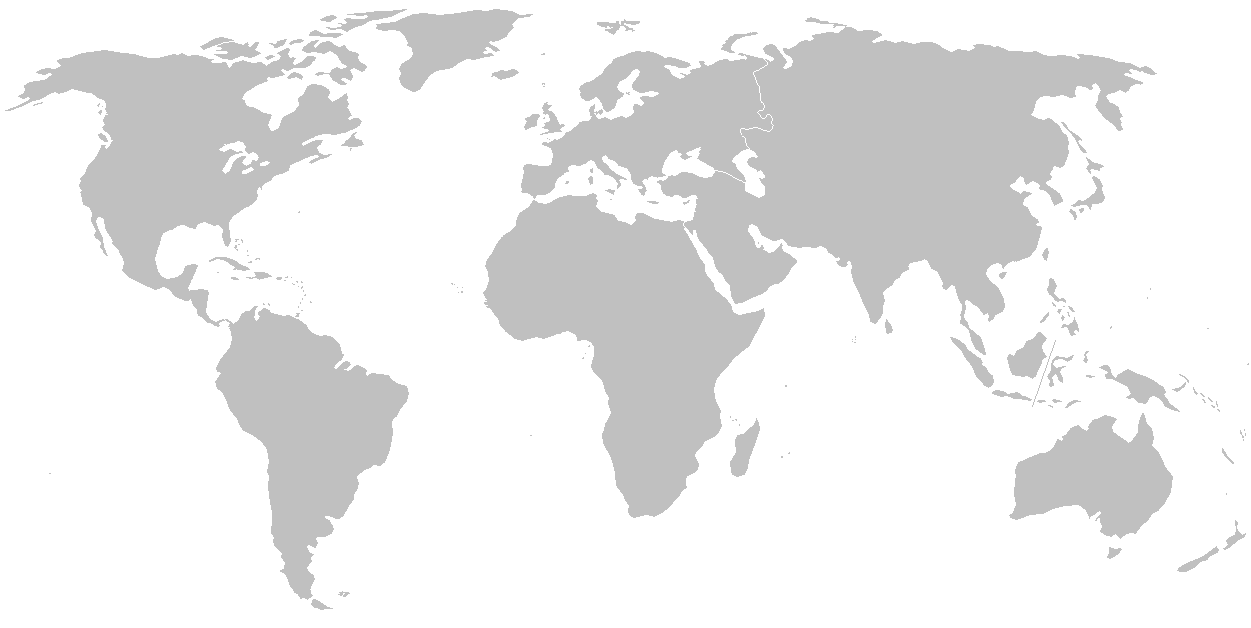
\includegraphics[width=\textwidth]{media/chapter2/continents.png}
\caption{Horizontal/vertical extents of different continents.}
\label{fig:continental-axis}
\end{figure}

There is also this idea that cultures which had to undergo such reboots frequently had to deal with more complexities of the world, and could rely less on objective knowledge, and therefore made people rely more on religious principles to lead their lives. This led to prevalence, and eventually domination by religious organizations.

% http://pocketcultures.com/topicsoftheworld/files/2009/06/map-importance-of-religion-by-country.png

% http://en.wikipedia.org/wiki/File:Religion_in_the_world.PNG

Diamond's book is an exploration of the broadest pattern of history. What it tells us is that explicit modeling of real world objects with their native properties are extremely important in reasoning about the world.

\subsection{The Gaia Hypothesis}
Charles Darwin's work describes how living being have evolved over billions on years. But it does not answer the question -- how does life sustain itself on Earth? It turns out that the few billion years of life we have had is too little to let life have grown randomly, and just let natural selection determine who succeeds. There had to be bigger factors which let life sustain and grow in specific ways.

One of the theories proposed in the 1970s is commonly known as the Gaia Theory. Proposed by James Lovelock and Lynn Margulis, it proposes the presence of feedback loops to explain the sustanence of life. Their argument is that for life to sustain, the amount of carbon dioxide in the atmosphere must not exceed a certain threshold. But who keeps this in check? How has the amount of $CO_2$ in the atmosphere been almost constant for the last millions of years. Their reasoning is as follows:

The Earth's volcanoes have spewed out huge amounts of carbon dioxide for millions of years. Plant and animals recycle massive amounts of $CO_2$ in the process of photosynthesis, respiration and decay. According to the Gaia theory, the excess of $CO_2$ is recycled is removed and recycled by a vast feedback loop, which involves rock weathering as a key ingredient. In the process of rock weathering, rocks, rainwater and $CO_2$ form chemicals known as carbonates which are taken out of the atomosphere and bound in liquid solutions. It turns out that soil bacteria vastly increases the rate of rock weathering. The carbonates are then washed down where tiny algae invisble to the naked eye, absorb them and use them to make shells of chalk. So the $CO_2$ that was in the atmosphere has now ended up in the shells of those minute algae. In addition, ocean algae also absorb $CO_2$ from the ocean.  

When the algae die their shells are then washed down into the ocean, where they form sediments of limestone. Limestone is very heavy, and gradually sinks into the mantle of the earth. Eventually, some of the $CO_2$ is released back to the atomsphere by volcanoes. The entire cycle -- linking volcanoes to rock weathering, to soil bacteria, to oceanic algae, to limestone sediments, and back to volcanoes -- acts as a feedback loop which regulates the Earth's temperature. As the sun gets hotter, the bacteria in the soil get hotter, and more $CO_2$ is removed from the atmosphere and sent to the ocean, thus cooling the planet.

This remarkable explanation involves rocks, bacteria and ocean dynamics and the even the sun to explain how the earth's temperature is regulated. By studying one or more objects in isolation makes the analysis far from complete. More interestingly, the relations between the objects are very precise, involving biochemical reactions and have very precise definitions.

\subsection{Significance}
The reason these examples are not to present the latest advances in different disciplines, but to glance at how reasoning is done in the real world. Both the use cases require very precise knowledge of relations between different objects in the world (for example, how the sun can affect bacterial growth in the soil), and have access to a large amount of sensors and data sources. Once these two have been established, the computational challenge is how to form accurate models of the models of the world, and how to use those models to either reduce the complexity of the problem so a human can operate with ease, or apply computational algorithms which directly solve the problem. 

In the next section, we see what we types of information we shall consider as context for the problem of tagging personal photos.

\section{Context for Personal Photos}
Our justification for the use of context begins with the statement: \textit{For a given user, the correctness of face tags for a photograph containing people she has never met is undefined}. This observation prepares us to understand what context is, and how contextual reasoning assists in tagging photos. The description of any problem domain requires a set of abstract data types, and a model of how these types are related to each other. We \textbf{define} contextual types as those which are semantically different from these data types, but can be directly or indirectly related to them via an extended model which encapsulates the original one. Contextual reasoning assists in the following two ways. \textbf{First}, contextual data restricts the number of people who might appear in the photographs. We can also argue that all the personal data of a user (her profile on Facebook, LinkedIn, email exchanges, phone call logs) provides a reasonable estimate of all these people who might appear in her photos. \textbf{Second}, by reasoning on abstractions in the contextual domain, we can infer conclusions on the original problem. We exploit this property to develop our algorithm in the later sections. Though CueNet can be applied to a variety of recognition problems, we focus on tagging people in personal photos for concreteness, where, the image and person tag form the abstractions in the problem domain. The types used in the contextual domain, but not limited to, are the following:

\begin{itemize}
\item \textbf{Events}: includes description of events like conferences, parties, trips or weddings, and their structure (for example, what kind of sessions, talks and keynotes are occurring within a particular conference).
\item \textbf{Social Relationships}: information about a user's social graph, people whom she corresponds with using email and other messaging services.
\item \textbf{Geographical Proximity}: various tools like Facebook Places, Google Latitude or Foursquare provide information about where people are at a given time.
\end{itemize}

The above classes of contextual data can be obtained from a variety of data sources. Examples of data sources range from mobile phone call logs and email conversations to Facebook messages to a listing of public events at upcoming.com. We classify sources into the following types:

\begin{itemize}
\item \textbf{Personal Data Sources}: include all sources which provide details about the particular user whose photo is to be tagged. Some common examples of personal data sources include Google Calendar, Email and Facebook profile and social graph.
\item \textbf{Social Data Sources}: include all sources which provide contextual information about a user's friends and colleagues. For example, LinkedIn, Facebook and DBLP are some of the commonly used websites with different types of social graphs.
\item \textbf{Public Data Sources}: include all sources which provide information about public organizations (like restaurants, points of interest or football stadiums) or about public events (like fairs, concerts or sports games).
\end{itemize}

Social and public data sources are enormous in size, containing information about billions of events and entities. Trying to use them directly will lead to scalability problems faced by face recognition and verification techniques. But, by using personal data, we can discover which parts of social and public sources are more relevant. For example, if a photo was taken at San Francisco, CA (where the user lives) his family in China is less relevant. Thus, the role of personal information is twofold. \textbf{Firstly}, it provides contextual information regarding the photo. \textbf{Secondly}, it acts as a bridge to connect to social and public data sources to discover interesting people connected to the user who might be present in the event and therefore, the photo.

At this point we should revisit the \textbf{temporal relevance} property of a data source. Given a stream of photos taken during a time interval, the source which contributed interesting context for a photo might not be equally useful for the one appearing next. This is because sources tend to focus on a specific set of event types or relationship types, and the two photos might be captured in different events or contains persons with whom the user maintains relations through different sources. For example, two photos taken at a conference might contain a user's friends in the first, but with advisers of these friends in the next. The friends might interact with the user through a social network, but their advisers might not. By using a source like DBLP, the relations between the adviser and friends can be discovered. We say that the temporal relevance of these context sources is \textbf{\textit{low}}. This requirement will play an important role in the design of our framework, as now, sources are not hardwired to photo, but instead need to be discovered gradually.

conclusion: by using events we get dynamic linking, temporal relevance and real world integration.



%\subsection{Zeno's Paradox}
% \textit{In the paradox of Achilles and the Tortoise, Achilles is in a footrace with the tortoise. Achilles allows the tortoise a head start of 100 metres, for example. If we suppose that each racer starts running at some constant speed (one very fast and one very slow), then after some finite time, Achilles will have run 100 metres, bringing him to the tortoise's starting point. During this time, the tortoise has run a much shorter distance, say, 10 metres. It will then take Achilles some further time to run that distance, by which time the tortoise will have advanced farther; and then more time still to reach this third point, while the tortoise moves ahead. Thus, whenever Achilles reaches somewhere the tortoise has been, he still has farther to go. Therefore, because there are an infinite number of points Achilles must reach where the tortoise has already been, he can never overtake the tortoise.}

% How can achilles win? Idea: Ignoring a variable can make a process very hard to explain. Different variables work together holistically. In this case, it is time. Just by bringing it into the same picture the problem becomes tractable.
